\documentclass{article}
\usepackage{fullpage}
\usepackage{color,soul}
\usepackage{amsmath}
\usepackage{url}
\usepackage{verbatim}
\usepackage{graphicx}
\usepackage{parskip}
\usepackage{amssymb}
\usepackage{nicefrac}
\usepackage{listings}
\usepackage{fancyvrb}
\usepackage{float}
\usepackage{transparent}

\graphicspath{ {./images/} }

% Colors
\definecolor{blu}{rgb}{0,0,1}
\def\blu#1{{\color{blu}#1}}
\definecolor{gre}{rgb}{0,.5,0}
\def\gre#1{{\color{gre}#1}}
\definecolor{red}{rgb}{1,0,0}
\def\red#1{{\color{red}#1}}
\definecolor{lblu}{RGB}{10,213,216}
\def\lblu#1{{\color{lblu}#1}}

\def\image#1#2{{\includegraphics[scale=#2]{#1}}}

%Template
%\definecolor{x}{rgb}{0,0,0}
%\def\x#1{\color{x}#1}
\setul{0.5ex}{0.3ex}
\setulcolor{red}
 
\def\norm#1{\|#1\|}

% LaTeX
\def\items#1{\begin{itemize}#1\end{itemize}}
\def\enum#1{\begin{enumerate}#1\end{enumerate}}


\begin{document}

\title{Website Development Notes}
\author{Muhammad Ali}
\date{}
\maketitle

\section{codeacademy: CSS}
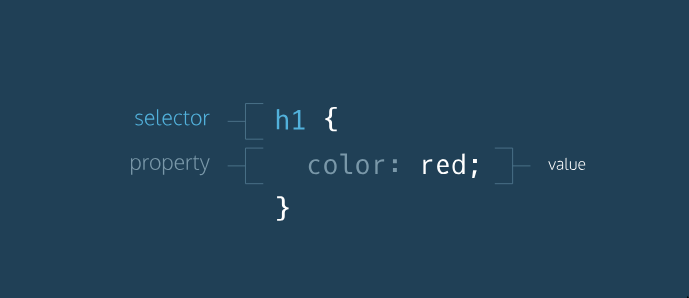
\includegraphics[scale=0.25]{css-outline.png}
\subsection{The box model}
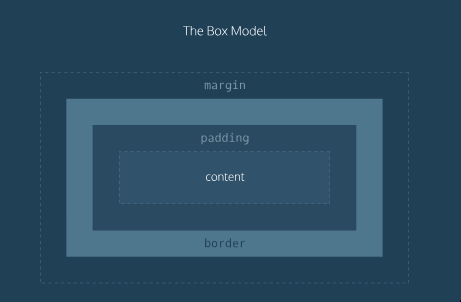
\includegraphics[scale=0.5]{box-model.png}

Content: includes text and other media \newline \newline
padding: \textit{as it looks like} \newline \newline
border: outline of an HTML page element. \textit{picture frame that contains the element}
use like \newline
\textbf{p \{ border: 2px [solid, dotted, dashed] [black, blue ...]\}} \newline \newline
margin: space b/w HTML page element and \textbf{next nearest element}. \newline
Also, doing something like \textit{p \{margin: 20px\}} will create spacings on each side of an element.\newline
You can do \textbf{margin-top, margin-bottom, margin-left, margin-right.}\newline \newline



\subsection{Block vs Inline Elements}
Allows to control the boundaries and space for individual HTML elements. It determines how HTML elements move around in the page.
\newline
\image{block-inline.png}{0.4}
\newline
\underline{These are properties for the css selector}\newline \newline
\ul{display:} [none, inline, block, inline-block]
\enum{
\item{\textbf{block:} HTML heading, paragraph, unordered list}
\item{\textbf{inline:} HTML image and anchor elements}
}
\ul{position:} [static, relative, fixed, absolute, sticky]
\enum{
\item{\textbf{static:} always positioned according to normal flow of page.}
\item{\textbf{relative:} Setting top, right bottom, and left properties of a "relative" positioned element will adjust it away from its normal position.\newline \image{relative.png}{0.3}}
\item{\textbf{fixed:} Just keeps some HTML element in the same place even when you're scrolling. You can use \textbf{top, bottom, right, left} to position it.\newline \image{fixed.png}{0.3}}
\item{\textbf{absolute:} positioned relative to the nearest positioned ancestor (instead of viewport like fixed)\newline \image{absolute.png}{0.3}}
\item{\textbf{sticky:} toggles between relative and fixed depending on the scroll position. Basically just follows you arround.\image{sticky.png}{0.3}}
}


\end{document}


